%% This is an example first chapter.  You should put chapter/appendix that you
%% write into a separate file, and add a line \include{yourfilename} to
%% main.tex, where `yourfilename.tex' is the name of the chapter/appendix file.
%% You can process specific files by typing their names in at the 
%% \files=
%% prompt when you run the file main.tex through LaTeX.

\chapter{Experimentos y Resultados}


\section{Experimentos}


\section{Resultados}

\begin{figure}[htp]
  \centerline{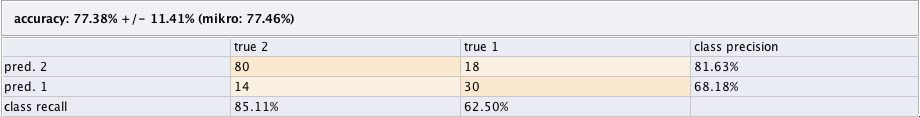
\includegraphics[width=16.09cm]{frustration-accuracy.png}} \caption{Precisión
    del modelo de clasificación para el estado mental de frustración.
} \label{frustration-accuracy}
\end{figure}

\begin{figure}[htp]
  \centerline{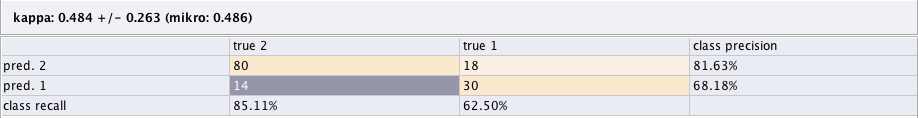
\includegraphics[width=16.09cm]{frustration-kappa.png}} \caption{Coeficiente
    de kappa del modelo de clasificación para el estado mental de frustración.
} \label{frustration-kappa}
\end{figure}


% boredom
\begin{figure}[htp]
  \centerline{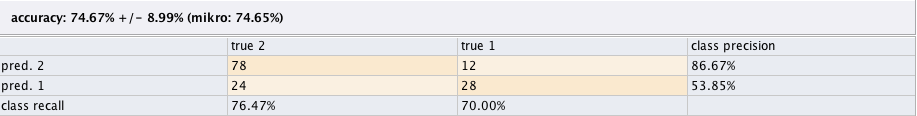
\includegraphics[width=16.09cm]{boredom-accuracy.png}} \caption{Precisión
    del modelo de clasificación para el estado mental de aburrimiento.
} \label{frustration-accuracy}
\end{figure}

\begin{figure}[htp]
  \centerline{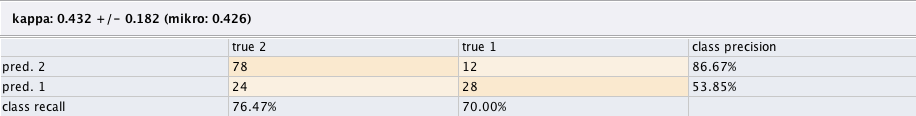
\includegraphics[width=16.09cm]{boredom-kappa.png}} \caption{Coeficiente
    de kappa del modelo de clasificación para el estado mental de aburrimiento.
} \label{frustration-kappa}
\end{figure}